\documentclass[12pt]{article}

\usepackage{enumerate}
\usepackage{amsmath}
\usepackage{amsthm}
\usepackage{amssymb}
\usepackage{changepage}
\usepackage{graphicx}
\usepackage[a4paper, margin=1in]{geometry}
\allowdisplaybreaks[1]

\title{DATA315 Assignment 3}
\author{Rin Meng 51940633}
\date{\today}

\begin{document}

\maketitle

\begin{enumerate}
    \item
    \begin{enumerate}
    \item
    \begin{verbatim}
source("nickel.R")
acf(nickel, lag.max = 10, 
main = "ACF of Electroless Nickel Concentrations")
     \end{verbatim}
    \begin{center}
        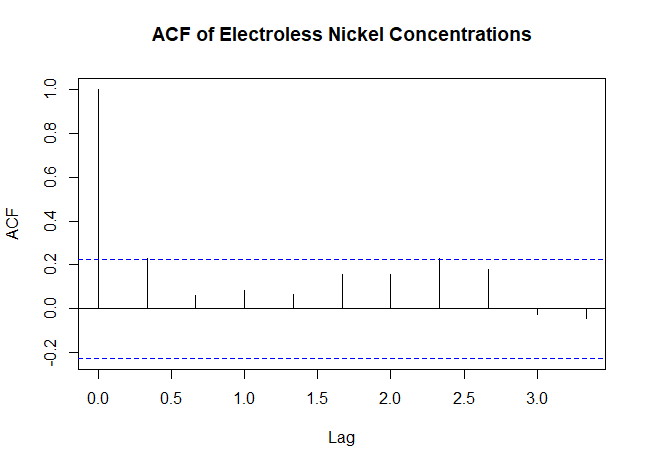
\includegraphics[width=0.8\textwidth]{Rplot.png}
    \end{center}
    The ACF plot seems to follow an MA(1) process,
    as significant correlation at lag 1 followed by immediate drop to near zero. 
    \item
\begin{verbatim}
data(lynx)
acf(lynx, lag.max = 10, main = "ACF of Lynx Trapping Data")
\end{verbatim}
    \begin{center}
        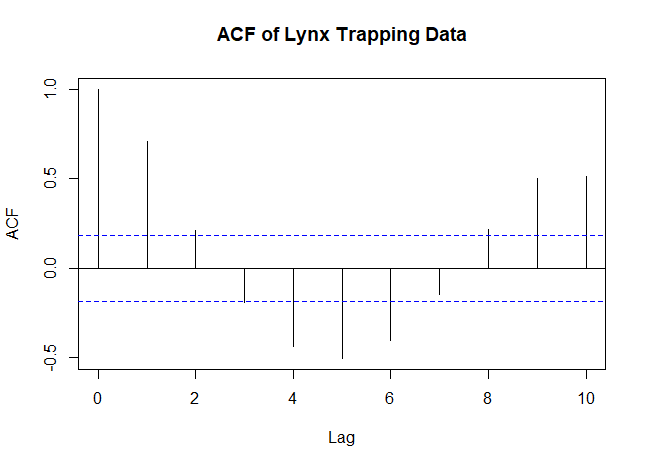
\includegraphics[width=0.8\textwidth]{Rplot01.png}
    \end{center}
    So far, there are no models that fit, because the plot shows a cyclic pattern between
    predator and prey populations. 
    \item
\begin{verbatim}
source("Globaltemps.R")
temps <- ts(temps, start = 1880, end = 2016)
acf(temps, lag.max = 10, 
main = "ACF of Global Average Temperatures")
\end{verbatim}
    \begin{center}
        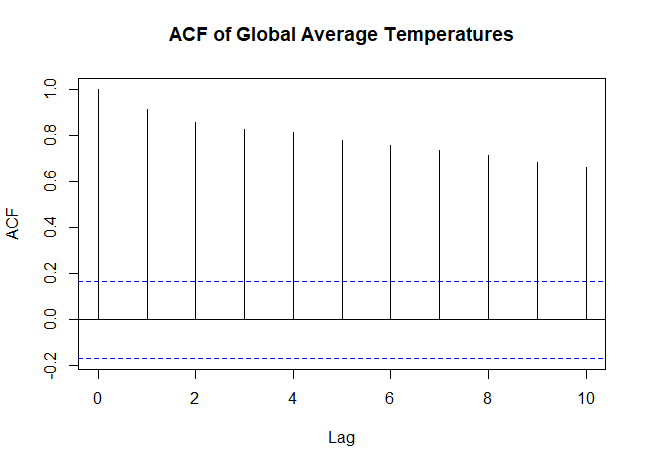
\includegraphics[width=0.8\textwidth]{Rplot02.png}
    \end{center}
    The ACF plot seems to follow an AR(1) process,
    as significant correlation at lag 1 followed by gradual decay.
    \item 
    \begin{verbatim}
data("EuStockMarkets")
dax <- EuStockMarkets[, 1]

# 260 trading days per year
dax_ts <- ts(dax, start = c(1991, 1), frequency = 260)

# Time series plot
plot(dax_ts, 
main = "DAX Stock Index Time Series", 
ylab = "Index Value", xlab = "Year", 
col = "blue", type = "l")

# ACF plot
acf(dax_ts, main = "ACF of DAX Stock Index")

# Take the natural log
log_dax <- log(dax_ts)
# Compute first differences (log returns)
diff_log_dax <- diff(log_dax)
acf(diff_log_dax, main = "ACF of Log Returns of DAX")
    \end{verbatim}
    \begin{center}
        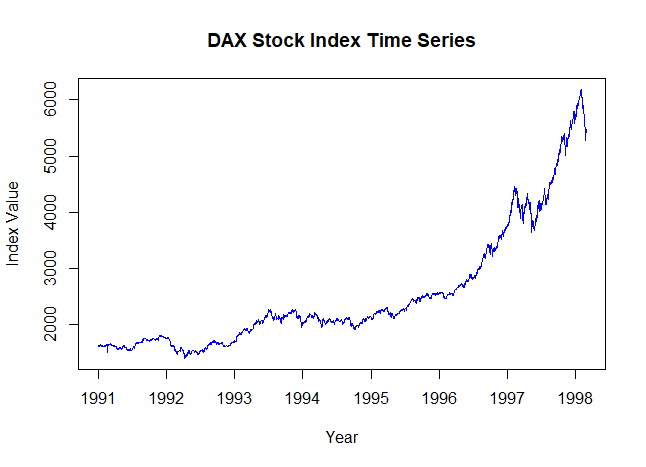
\includegraphics[width=0.8\textwidth]{Rplot03.png}
        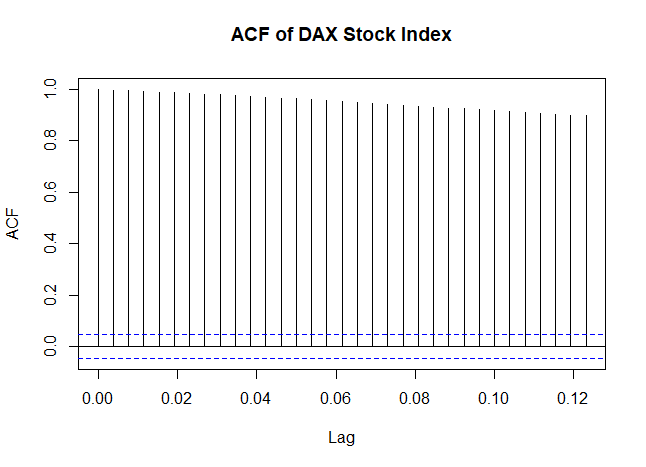
\includegraphics[width=0.8\textwidth]{Rplot04.png}
        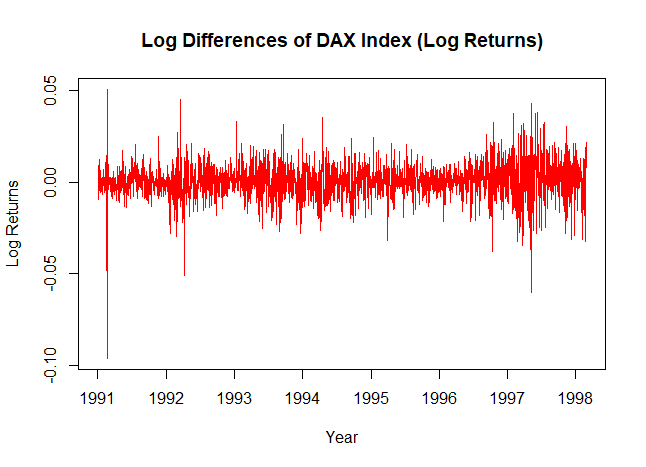
\includegraphics[width=0.8\textwidth]{Rplot05.png}
    \end{center}
    Some observations for the DAX stock index time series plot; visually, we can see that
    there is a general upward trend with some fluctuations. The ACF plot shows that there is
    a significant correlation at lag 1, followed by a gradual, slow decay, which means that it
    may be following other process we have not covered yet. The log returns plot shows that 
    the data revolves around 0, which is a good sign for stationarity.
    \end{enumerate} 
    \item
    \begin{enumerate}
    \item Given that the MA(1) process is defined as
    \[
        X_t = \mu_t + \epsilon_t + \theta \epsilon_{t-1}
    \]
    Now we have to test whether the MA parameter is equal 
    to 0.
\begin{verbatim}
# Print the model summary
summary(ma1_model)

Call:
arima(x = nickel, order = c(0, 0, 1))

Coefficients:
            ma1  intercept
        0.2260     4.6223
s.e.  0.1099     0.0277

sigma^2 estimated as 0.03857:  
log likelihood = 15.63,  aic = -25.26

# Extract MA(1) coefficient and its standard error
theta_hat <- ma1_model$coef["ma1"]
se_theta <- sqrt(ma1_model$var.coef["ma1", "ma1"])

# Compute t-statistic
t_value <- theta_hat / se_theta

# Compute p-value (two-tailed test)
p_value <- 2 * (1 - pnorm(abs(t_value)))

# Print results
t_value
    ma1 
2.05681 
p_value
    ma1 
0.03970446
\end{verbatim}
    The fitted model is $X_t = 4.6223 + \epsilon_t + 0.2260 \epsilon_{t-1}$.
    Since the p-value is less than 0.05, we reject the null hypothesis that the MA parameter is equal to 0.
    Forecasting the 2nd and 3rd values after the end of the series, we can use
    \[
        X_{t+1} = 4.6223 + \epsilon_{t+1} + 0.2260 \epsilon_t
    \]
    \[
        X_{t+2} = 4.6223 + \epsilon_{t+2} + 0.2260 \epsilon_{t+1}
    \]
    \item The portmanteau test checks whether the residuals
    from our fitted MA(1) model behave like white noise, meaning they are uncorrelated.
    We can use the Box-Ljung test to check this.
\begin{verbatim}
# Perform the Box-Ljung test
Box.test(ma1_model$residuals, lag = 10, type = "Ljung-Box")

library(forecast)
checkresiduals(ma1_model)

Ljung-Box test

data:  Residuals from ARIMA(0,0,1) with non-zero mean
Q* = 2.5221, df = 5, p-value =
0.7732

Model df: 1.   Total lags used: 6
\end{verbatim}
    Since the p-value is greater than 0.05, we fail to reject the null hypothesis that the residuals are uncorrelated.
    \item If the 75th value is missing, we can forecast it using the fitted
    MA(1) model.
    \[
        X_{75} = 4.6223 + \epsilon_{75} + 0.2260 \epsilon_{74}
    \]
    Now we can extract the last residuals
\begin{verbatim}
# Extract last residual
epsilon_74 <- residuals(ma1_model)[74]

# Compute forecast
X_75_hat <- 4.6223 + (0.2260 * epsilon_74)
X_75_hat
[1] 4.545646
\end{verbatim}
    The forecasted value for $X_{75}$ is 4.545646.
    The standard deviation of the forecast is given by
    \[
        \sigma_{\text{forecast}} = \sqrt{\hat{\sigma}^2} \sqrt{1 + \theta^2}
    \]
    From the model, we have 
    \[
        \hat{\sigma}^2 = 0.03857
    \]
    \[
        \theta = 0.2260
    \]
    So we can calculate the standard deviation of the forecast.
    \[
        \sigma_{\text{forecast}} = \sqrt{0.03857} \sqrt{1 + 0.2260^2} = 0.2013455
    \]
    The error in terms of standard deviations is given by
    \[
        Z = \frac{X_{75} - X_{75}^{\text{forecast}}}{\sigma_{\text{forecast}}}
        = \frac{4.3 - 4.545646}{0.2013455} = -1.220022
    \]
    Since $|Z| < 2$, the forecast is within the 95\% confidence interval.

    \item First we fit an AR(1) model to the data.
\begin{verbatim}
ar1_model <- arima(nickel, order = c(1, 0, 0))

# Print model summary
summary(ar1_model)

Call:
arima(x = nickel, order = c(1, 0, 0))

Coefficients:
            ar1  intercept
        0.2363     4.6221
s.e.  0.1139     0.0295

sigma^2 estimated as 0.03845:  
log likelihood = 15.74,  aic = -25.47
\end{verbatim}
    Then we forecast for the 2nd and 3rd values after the end of
    the series.
\begin{verbatim}
# Forecast 2 steps ahead
ar1_forecast <- predict(ar1_model, n.ahead = 3)

# Print forecasted values
ar1_forecast$pred
Time Series:
Start = c(26, 1) 
End = c(26, 3) 
Frequency = 3 
[1] 4.545956 4.604083 4.617820
\end{verbatim} 
    Now we check if the residuals are white noise.
\begin{verbatim}
# Perform Ljung-Box test on AR(1) residuals
Box.test(ar1_model$residuals, lag = 10, type = "Ljung-Box")

Box-Ljung test

data:  ar1_model$residuals
X-squared = 7.1631, df = 10, p-value = 0.71
\end{verbatim}
    Since the p-value is greater than 0.05, 
    we fail to reject the null hypothesis that the 
    residuals are white noise.
    \end{enumerate}
    \item The given time series model is
    \[
        y_t = \mu + \phi(y_{t-1} - \mu) + \varepsilon_t
    \]
    The exepected value of $y_t$ is
    \[
        E(y_t) = \mu + \phi(E(y_{t-1}) - \mu)
    \]
    \[
       = \mu + \phi(\mu - \mu) = \mu
    \]
    $\mu$ can be estimated by the sample mean:
    \[
        \hat{\mu} = \frac{1}{n} \sum_{t=1}^{n} y_t
    \]
    for the given data $\{3.2,3.2,2.2,2.3,1.8,1.3,2.2,2.7\}$
    \[
        \hat{\mu} = \frac{1}{8} (3.2 + 3.2 + 2.2 + 2.3 + 1.8 + 1.3 + 2.2 + 2.7) = 2.3625
    \]
    \[
        \hat{\mu} = 2.3625
    \]
    Now, we will estimate $\phi$.
    The autocovariance at lag 1 is given by
    \[
        \gamma_1 = E[(y_t - \mu)(y_{t-1} - \mu)]
    \]
    which can be estimated by
    \[
        \hat{\gamma}_1 = \frac{1}{n} \sum_{t=2}^{n} (y_t - \hat{\mu})(y_{t-1} - \hat{\mu})
    \]
    similarly, the vairance its
    \[
        \gamma_0 = E[(y_t - \mu)^2]
    \]
    which can be estimated by
    \[
        \hat{\gamma}_0 = \frac{1}{n-1} \sum_{t=1}^{n} (y_t - \hat{\mu})^2
    \]
    Sine for this process, the autocorrealtion at lag 1 is given by
    we can estimate $\phi$ by
    \[
        \hat{\phi} = \frac{\hat{\gamma}_1}{\hat{\gamma}_0}
    \]
    Computing the estimates for $\gamma_1$ and $\gamma_0$:
    \[ 
    \hat{\gamma}_0 = \frac{1}{8} 
    \sum_{t=1}^{8} (y_t - 2.3625)^2 = 0.3773438
    \]
    \[
    \hat{\gamma}_1 = \frac{1}{8}
    \sum_{t=2}^{8} (y_t - 2.3625)(y_{t-1} - 2.3625) = 0.189442
    \]
    So the estimate for $\phi$ is
    \[
        \hat{\phi} = \frac{0.189442}{0.3773438} = 0.502
    \]
    Now we can estimate $\sigma$ by
    \[
        \hat{\sigma}^2 = \hat{\gamma}_0(1 - \hat{\phi}^2) = 0.282
    \]
    \[    
        \hat{\sigma} = \sqrt{0.282} = 0.531
    \]

    \item 
    \begin{verbatim}
# Compute and display ACF
library(RCMinification)
# Load the data
acf_values <- acf(longitudinalAcceleration, 
                lag.max = 4, plot = FALSE)

# Extract the first lag autocorrelation
# First lag autocorrelation (index 2 because index 1 is lag 0)
rho_1 <- acf_values$acf[2]

# Compute theoretical autocorrelations
rho_2 <- rho_1^2
rho_3 <- rho_1^3
rho_4 <- rho_1^4

# Extract sample autocorrelations
sample_rho_2 <- acf_values$acf[3]
sample_rho_3 <- acf_values$acf[4]
sample_rho_4 <- acf_values$acf[5]

# Print comparisons
cat("Theoretical vs. Sample Autocorrelations:\n")
cat(sprintf("Lag 2: Theoretical = %.4f, 
            Sample = %.4f\n", rho_2, sample_rho_2))
cat(sprintf("Lag 3: Theoretical = %.4f, 
            Sample = %.4f\n", rho_3, sample_rho_3))
cat(sprintf("Lag 4: Theoretical = %.4f, 
            Sample = %.4f\n", rho_4, sample_rho_4))

# Printed output
Theoretical vs. Sample Autocorrelations:
Lag 2: Theoretical = 0.0201, Sample = 0.0689
Lag 3: Theoretical = 0.0028, Sample = 0.0141
Lag 4: Theoretical = 0.0004, Sample = 0.0221
    \end{verbatim}
    Since the sample autocorrelations are greater than the theoretical autocorrelations (in many deviations),
    then this data is not consistent for an AR(1) model, also, if it was AR(1), there would have been a decay
    pattern in the ACF, which is not the case here.
    
    \item Given the TS
    \[ x_t = 0.5x_{t-1} \]
    for $t = 1,2, \ldots, n$ and $x_0 = 0$.

    \begin{enumerate}
        \item $x_1$ and $x_2$ can be found by,
        \[ x_1 = 0.5x_0 = 0.5(0) = 0 \]
        \[ x_2 = 0.5x_1 = 0.5(0) = 0 \]
        \item A formula for $x_t$ in terms of $t$ is
        \[ x_t = 0 \]
        \item The $\lim_{t \to \infty} x_t$ is
        \[ \lim_{t \to \infty} x_t = 0 \]
        \item Repeating (a), (b), and (c) for where $x_0 = 1$.
        \[ x_1 = 0.5x_0 = 0.5(1) = 0.5 \]
        \[ x_2 = 0.5x_1 = 0.5(0.5) = 0.25 \]
        \[ \lim_{t \to \infty} x_t = 0 \]
        because of geometric sequence convergence.
    \end{enumerate}

    \item Given that $x_0 = 10$ and 
    \[ x_t = 0.8x_{t-1} \] for $t = 1, 2, 3, \ldots, n$.

    \begin{enumerate}
        \item $x_1, x_2, x_3, x_4$ can be found,
        \[ x_1 = 0.8x_0 = 0.8(10) = 8 \]
        \[ x_2 = 0.8x_1 = 0.8(8) = 6.4 \]
        \[ x_3 = 0.8x_2 = 0.8(6.4) = 5.12 \]
        \[ x_4 = 0.8x_3 = 0.8(5.12) = 4.096 \]
        \item A formula for $x_t$ in terms of $t$ is
        \[ x_t = 10(0.8)^t \]
        \item The $\lim_{t \to \infty} x_t$ is
        \[ \lim_{t \to \infty} x_t = 0 \]
        \item Sketching the plot of $x_t$ vs. 
        $x_{t-1}$ for $t = 1, 2, 3, \ldots, 10$
        \begin{verbatim}
# Initial value
x0 <- 10

# Part (a): Compute the sequence xt = 0.8 * xt-1
t_values <- 0:10
x_values <- numeric(length(t_values))
x_values[1] <- x0

for (t in 2:length(t_values)) {
    x_values[t] <- 0.8 * x_values[t-1]
}

# Extract x_t and x_{t-1}
x_t <- x_values[-1]  # Remove x0
x_t_minus_1 <- x_values[-length(x_values)]  # Remove last value

# Plot x_t vs. x_{t-1}
plot(x_t_minus_1, x_t, type="b", col="blue", pch=16, 
xlab="x_{t-1}", ylab="x_t", main="x_t vs. x_{t-1}")

\end{verbatim}
        \begin{center}
            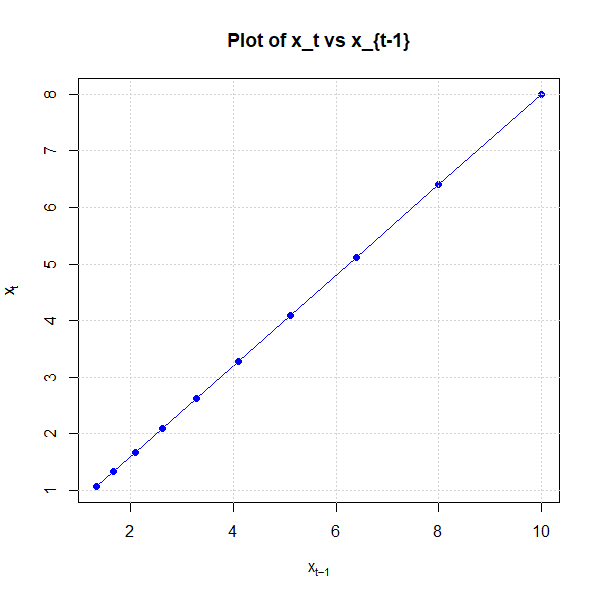
\includegraphics[width=0.7\textwidth]{Rplot06.png}
        \end{center}
        \item Sketching the plot of $x_t$ vs. 
        $x_{t-2}$ for $t = 2, 3, 4, \ldots, 10$
\begin{verbatim}
# Part (e): Plot x_t vs. x_{t-2}
x_t_minus_2 <- x_values[-c(length(x_values), 
length(x_values)-1)]  # Remove last two
x_t_2 <- x_values[-c(1,2)]  # Remove first two

plot(x_t_minus_2, x_t_2, type="b", col="red", pch=16, 
xlab="x_{t-2}", ylab="x_t", main="x_t vs. x_{t-2}")
\end{verbatim}
        \begin{center}
            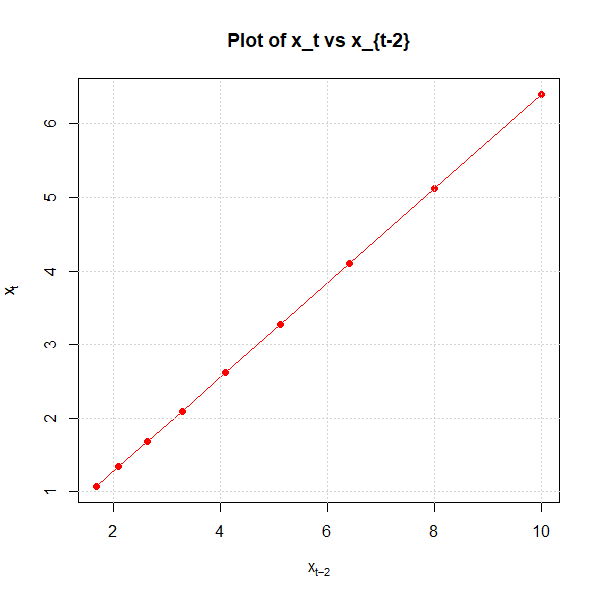
\includegraphics[width=0.7\textwidth]{Rplot07.png}
        \end{center}
        \item Repeating (a), (b), (c), (d), and (e) for 
        \[ x_t = 0.8x_{t-1} + z_t \]
        where $z_t, \ldots, z_n$ take on the values
        \[ \{ -1.2, 0.2, -1.0, 0.5, 1.7, -0.5, -2.1, 1.0, 0.8, -0.1 \}\]
        \begin{enumerate}
            \item $x_1, x_2, x_3, x_4$ can be found,
            \[ x_1 = 0.8x_0 + z_1 = 0.8(10) - 1.2 = 8 - 1.2 = 6.8 \]
            \[ x_2 = 0.8x_1 + z_2 = 0.8(6.8) + 0.2 = 5.44 + 0.2 = 5.64 \]
            \[ x_3 = 0.8x_2 + z_3 = 0.8(5.64) - 1.0 = 4.512 - 1.0 = 3.512 \]
            \[ x_4 = 0.8x_3 + z_4 = 0.8(3.512) + 0.5 = 2.8096 + 0.5 = 3.3096 \]
            \item A formula for $x_t$ in terms of $t$ is
            \[ x_t = 10(0.8)^t + \sum_{i=1}^{t} z_i \]
            \item The $\lim_{t \to \infty} x_t$ is
            \[ \lim_{t \to \infty} x_t = 0 \]
            \item Sketching the plot of $x_t$ vs.
            $x_{t-1}$ for $t = 1, 2, 3, \ldots, 10$
\begin{verbatim}
# Part (f): Compute the noisy sequence xt = 0.8 * xt-1 + zt
z_values <- c(-1.2, 0.2, -1.0, 0.5, 1.7, 
-0.5, -2.1, 1.0, 0.8, -0.1)
x_values_noise <- numeric(length(t_values))
x_values_noise[1] <- x0

for (t in 2:length(t_values)) {
x_values_noise[t] <- 0.8 * x_values_noise[t-1] 
+ z_values[t-1]
}

# Extract x_t and x_{t-1} for noisy data
x_t_noise <- x_values_noise[-1]
x_t_minus_1_noise <- x_values_noise[-length(x_values_noise)]

plot(x_t_minus_1_noise, x_t_noise, type="b", 
col="green", pch=16, 
xlab="x_{t-1}", ylab="x_t", 
main="x_t vs. x_{t-1} with noise")
\end{verbatim}
            \begin{center}
                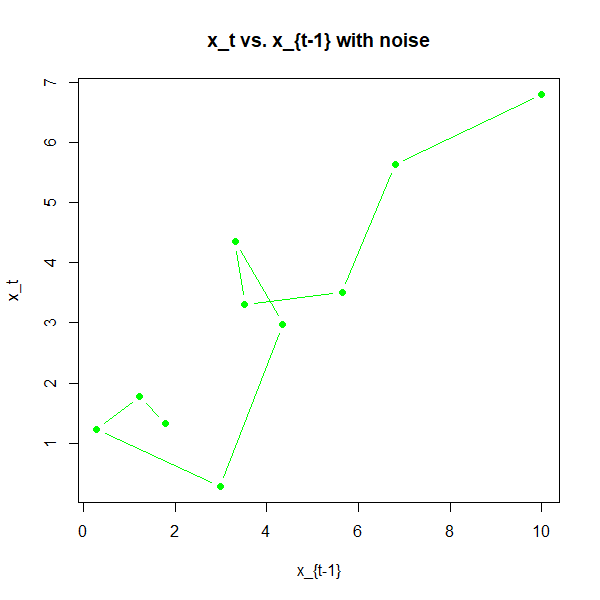
\includegraphics[width=0.7\textwidth]{Rplot08.png}
            \end{center}
            \item Sketching the plot of $x_t$ vs.
            $x_{t-2}$ for $t = 2, 3, 4, \ldots, 10$
\begin{verbatim}
# Part (e) with noise: x_t vs. x_{t-2}
x_t_minus_2_noise <- 
x_values_noise[-c(length(x_values_noise),
 length(x_values_noise)-1)]
x_t_2_noise <- x_values_noise[-c(1,2)]

plot(x_t_minus_2_noise, x_t_2_noise, type="b", 
col="purple", pch=16, 
xlab="x_{t-2}", ylab="x_t", 
main="x_t vs. x_{t-2} with noise")
\end{verbatim}
            \begin{center}
                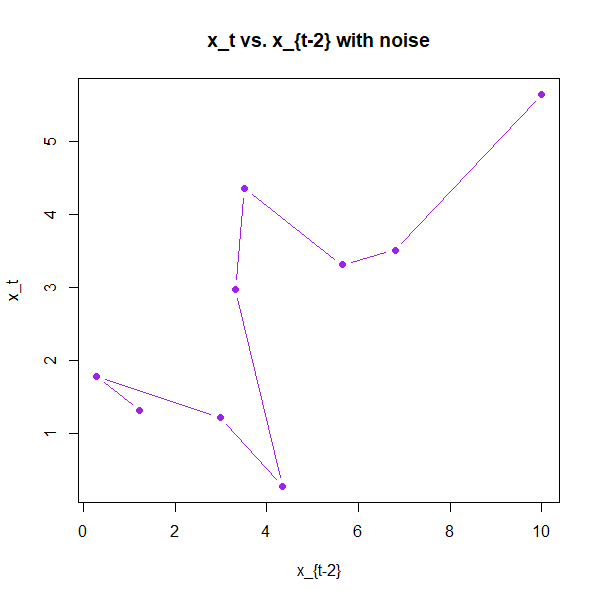
\includegraphics[width=0.7\textwidth]{Rplot09.png}
            \end{center}
        \end{enumerate}

    \end{enumerate}

    \item Given that $x_0 = 2$ and $x_1 = 1$ for
    \[ x_t = 0.8x_{t-1} - 0.7x_{t-2} \]
    for $t = 2, 3, 4, \ldots, n$
    \begin{enumerate}
        \item $x_2, x_3, x_4$ can be found,
        \[ 
        x_2 = 0.8x_1 - 0.7x_0 = 0.8(1) - 0.7(2) 
        = 0.8 - 1.4 = -0.6
        \]
        \[
        x_3 = 0.8x_2 - 0.7x_1 = 0.8(-0.6) - 0.7(1)
        = -0.48 - 0.7 = -1.18
        \]
        \[
        x_4 = 0.8x_3 - 0.7x_2 = 0.8(-1.18) - 0.7(-0.6)
        = -0.944 - (-0.42) = -0.524
        \]
        \item The sketched plot of $x_t$ vs. $x_{t-1}$ is
        for $t = 2, 3, \ldots, 10$ is shown below.
\begin{verbatim}
# Initial conditions
x_values <- numeric(11)
x_values[1] <- 2  # x0
x_values[2] <- 1  # x1

# Compute xt for t = 2 to 10 using 
# recurrence relation xt = 0.8*xt-1 - 0.7*xt-2
for (t in 3:11) {
x_values[t] <- 0.8 * x_values[t-1] - 0.7 * x_values[t-2]
}

# Extract values for plotting
x_t <- x_values[3:11]      # From t=2 to 10
x_t_minus_1 <- x_values[2:10]  # From t=1 to 9
x_t_minus_2 <- x_values[1:9]   # From t=0 to 8

# Plot x_t vs. x_{t-1}
plot(x_t_minus_1, x_t, type="b", col="blue", pch=16,
xlab="x_{t-1}", ylab="x_t", main="x_t vs. x_{t-1}")
\end{verbatim}
        \begin{center}
            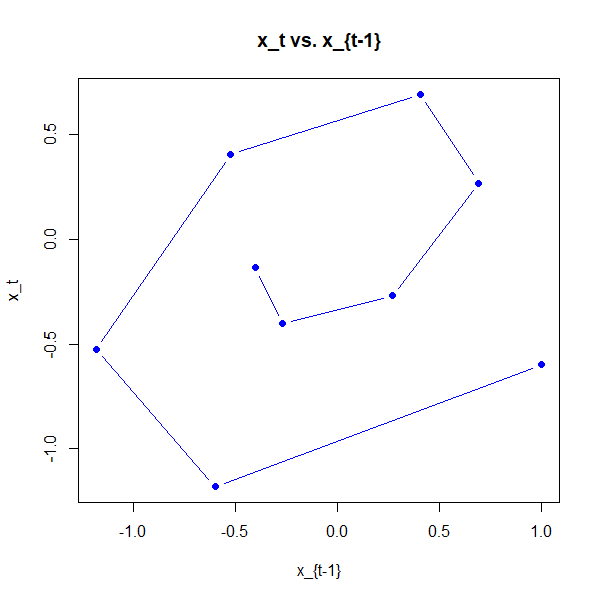
\includegraphics[width=0.7\textwidth]{Rplot10.png}
        \end{center}
        \item The sketched plot of $x_t$ vs. $x_{t-2}$ is
        for $t = 2, 3, \ldots, 10$ is shown below.
\begin{verbatim}
# Plot x_t vs. x_{t-2}
plot(x_t_minus_2, x_t, type="b", col="red", pch=16,
xlab="x_{t-2}", ylab="x_t", main="x_t vs. x_{t-2}")
\end{verbatim}
        \begin{center}
            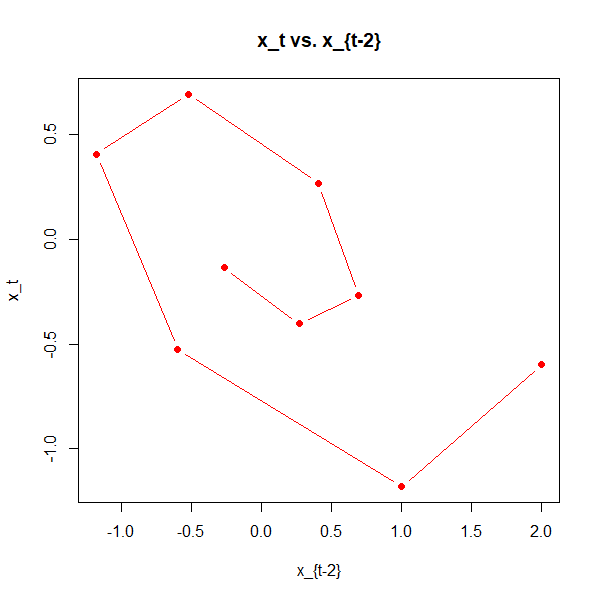
\includegraphics[width=0.7\textwidth]{Rplot11.png}
        \end{center}
        \item Repeat (a), (b), and (c) for
        \[ x_t = 0.8x_{t-1} - 0.7x_{t-2} + z_t \]
        where $z_2, \ldots, z_{11}$ take on the values
        \[ 
        \{ -1.2, 0.2, -1.0, 0.5, 1.7, -0.5, -2.1, 1.0, 0.8, -0.1 \} 
        \]
        \begin{enumerate}
            \item $x_2, x_3, x_4$ can be found,
            \[ 
            x_2 = 0.8x_1 - 0.7x_0 + z_2 
            = 0.8(1) - 0.7(2) + 0.2
            = 0.8 - 1.4 + 0.2 = -0.4
            \]
            \[
            x_3 = 0.8x_2 - 0.7x_1 + z_3 
            \]
            \[
            = 0.8(-0.4) - 0.7(1) - 1.0
            = -0.32 - 0.7 - 1.0 = -2.02
            \]
            \[
            x_4 = 0.8x_3 - 0.7x_2 + z_4  
            \]
            \[
            = 0.8(-2.02) - 0.7(-0.4) + 0.5
            = -1.616 - 0.28 + 0.5 = -1.396
            \]
            \item The sketched plot of $x_t$ vs. $x_{t-1}$ is
            for $t = 2, 3, \ldots, 10$ is shown below.
\begin{verbatim}
# Part (d): Compute with noise
z_values <- c(-1.2, 0.2, -1.0, 0.5, 1.7, 
-0.5, -2.1, 1.0, 0.8, -0.1)
x_values_noise <- numeric(11)
x_values_noise[1] <- 2
x_values_noise[2] <- 1

for (t in 3:11) {
x_values_noise[t] <- 0.8 * x_values_noise[t-1] 
- 0.7 * x_values_noise[t-2] + z_values[t-2]
}

# Extract noisy values
x_t_noise <- x_values_noise[3:11]
x_t_minus_1_noise <- x_values_noise[2:10]
x_t_minus_2_noise <- x_values_noise[1:9]

# Plot x_t vs. x_{t-1} with noise
plot(x_t_minus_1_noise, x_t_noise, type="b", 
col="green", pch=16,
xlab="x_{t-1}", ylab="x_t", 
main="x_t vs. x_{t-1} with noise")
\end{verbatim}
            \begin{center}
                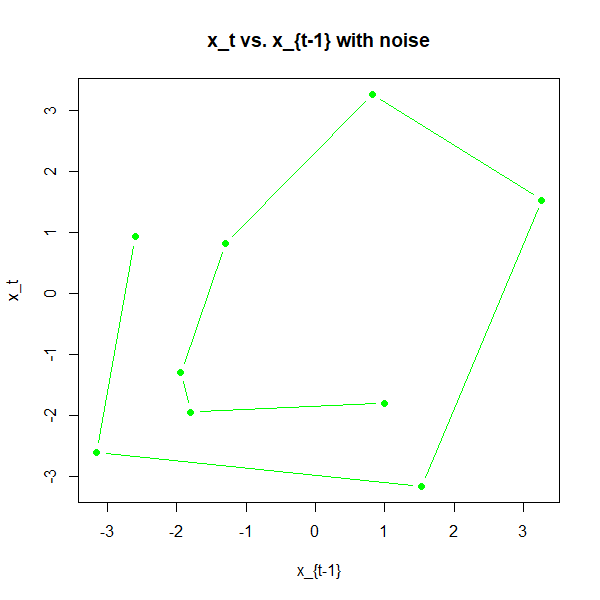
\includegraphics[width=0.7\textwidth]{Rplot12.png}
            \end{center}
            \item The sketched plot of $x_t$ vs. $x_{t-2}$ is
            for $t = 2, 3, \ldots, 10$ is shown below.
\begin{verbatim}
# Plot x_t vs. x_{t-2} with noise
plot(x_t_minus_2_noise, x_t_noise, type="b", col="purple", pch=16,
xlab="x_{t-2}", ylab="x_t", main="x_t vs. x_{t-2} with noise")
\end{verbatim}
            \begin{center}
                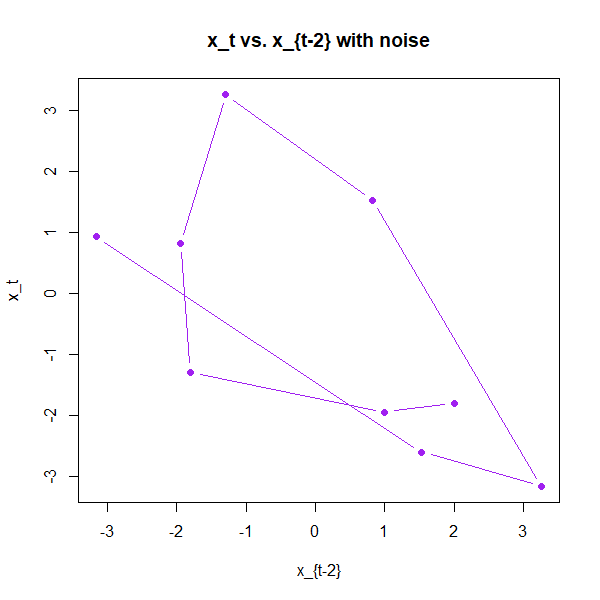
\includegraphics[width=0.7\textwidth]{Rplot13.png}
            \end{center}
        \end{enumerate}
    \end{enumerate}
    \item The given TS
    \[ x_t = 0.8x_{t-1} + z_t \]
    $z_t \sim N(0, 1)$ and $x_0 = 0$.
    \begin{enumerate}
        \item The distribution of $x_1$ its
        \[ x_1 = 0.8x_0 + z_1 = 0.8(0) + z_1 = z_1 \]
        \[ E[x_1] = 0 \]
        \[ Var[x_1] = 1 \]
        Since $z_1 \sim N(0, 1)$, $x_1 \sim N(0, 1)$.
        \item The distribution of $x_2$ is
        \[ x_2 = 0.8x_1 + z_2 = 0.8z_1 + z_2 \]
        \[ E[x_2] = 0 \]
        \[ 
        Var[x_2] = Var(0.8x_1) + Var(z_2) 
        = 0.8^2(1) + 1 = 1.64 
        \]
        Since $z_1, z_2 \sim N(0, 1)$, $x_2 \sim N(0, 1.64)$.
        \item The distribution of $x_3$ is
        \[ x_3 = 0.8x_2 + z_3 = 0.8(0.8z_1 + z_2) + z_3 \]
        \[ = 0.64z_1 + 0.8z_2 + z_3 \]
        \[ E[x_3] = 0 \]
        \[ 
        Var[x_3] = Var(0.8z_2) + Var(z_3) 
        =  0.8^2(1.64) + 1 = 2.0496 
        \]
        Since $z_1, z_2, z_3 \sim N(0, 1)$, $x_3 \sim N(0, 2.0496)$.
        \item If $x_2$ takes the value 3, the point prediction for $x_3$ is
        \[ E[x_3 | x_2 = 3] = 0.64(0) + 0.8(3) = 2.4 \]
        \item The distribution of the prediction error its
        \[ \text{Error} = x_3 - E[x_3 | x_2] \]
        Since $x_3 = 0.8x_2 + z_3$ and $E[x_3 | x_2] = 0.8x_2$,
        \[ \text{Error} = (0.8x_2 + z_3) - 0.8x_2 = z_3 \]
        then it must be true that 
        \[ \text{Error} \sim N(0, 1) \]
    \end{enumerate}
    \item \begin{enumerate}
        The AR(1) model with mean 0 is given by
    \[ x_t = \phi x_{t-1} + z_t \]
    where $z_t \sim N(0, \sigma^2)$.
    Then it must be true that the matrix form looks something like this
    \[
    \begin{bmatrix}
        x_1 \\
        x_2 \\
        x_3 \\
        \vdots \\
        x_n
    \end{bmatrix}
    =
    \begin{bmatrix}
        \phi & 0 & 0 & \cdots & 0 \\
        1 & \phi & 0 & \cdots & 0 \\
        0 & 1 & \phi & \cdots & 0 \\
        \vdots & \vdots & \vdots & \ddots & \vdots \\
        0 & 0 & 0 & \cdots & \phi
    \end{bmatrix}
    \begin{bmatrix}
        x_0 \\
        x_{1} \\
        x_{2} \\
        \vdots \\
        x_{n-1}
    \end{bmatrix}
    +
    \begin{bmatrix}
        \epsilon_1 \\
        \epsilon_2 \\
        \epsilon_3 \\
        \vdots \\
        \epsilon_n
    \end{bmatrix}
    \]
    The backshift operator $B$ is defined as
    \[ Bx_t = x_{t-1} \]
    then, the AR(1) model can be written as
    \[ e_t = x_t - \phi x_{t-1} \]
    \[ (1 - \phi B)x_t = e_t \]
    \item Yes, any process can be written in terms of $\epsilon_t$.
    An AR(1) is a process that can be express as a sum of
    past shocks $\epsilon_t$, if we write it recursively,
    \[ x_t = \phi x_{t-1} + \epsilon_t \]
    Substituting $x_{t-1} = \phi x_{t-2} + \epsilon_{t-1}$,
    \[ x_t = \phi(\phi x_{t-2} + \epsilon_{t-1}) + \epsilon_t \]
    \[ = \phi^2 x_{t-2} + \phi \epsilon_{t-1} + \epsilon_t \]
    Repeating this, we can get
    \[ x_t = \sum_{k=0}^{\infty} \phi^k \epsilon_{t-k} \]
    and this sum converges if $|\phi| < 1$, but if
    $|\phi| < 1$, then the process is stationary,
    and the sum can be fully written in terms of $\epsilon_t$.
    If $|\phi| \geq 1$, then the process is non-stationary,
    and the sum does not converge, whcih cannot be fully
    written in terms of $\epsilon_t$.
    \end{enumerate}
    
\end{enumerate}
\end{document}
